\chapter{Medidas y errores}

\section{Introducci'on}

En F'isica, y en general en Ciencias, no es posible determinar en forma 'unica, con infinita precisi'on, el valor de una magnitud f'isica por medio de un experimento. Todo experimento tiene asociado alg'un grado de error, variabilidad, o incertidumbre. Por esto, en la pr'actica no s'olo es relevante conocer el valor de una cierta magnitud, sino tambi'en la precisi'on con la que se determina este valor. 

Por ejemplo, el resultado de un experimento que permita medir la aceleraci'on de gravedad en alg'un lugar particular de la Tierra podr'a expresarse en la forma ``$x\pm\Delta x$"\, como
\begin{equation}
g = (9.70\pm 0.15) {\rm m/s^2}
\end{equation}
M'as adelante discutiremos con mayor profundidad lo que el ``error"\, $\pm 0.15\rm \,m/s^2$ significa, pero por ahora es suficiente enfatizar que este valor determina un rango de valores en el que consideramos que el experimento determina el valor de $g$: entre $(9.70-0.15)\,{\rm m/s^2} = 9.55\,{\rm m/s^2}$ y $(9.70+0.15)\,{\rm m/s^2} = 9.85 \,{\rm m/s^2}$, con alg'un grado de confianza (es decir, una cierta probabilidad. Por ahora, suponga que se tiene completa certeza que el valor de $g$ est'a en ese intervalo, es decir, 100\% de probabilidad que el valor medido est'a dentro del rango). Entre m'as peque\~no sea el valor de este error, m'as precisa ser'a la medida reportada.

Una de las razones por las que debemos considerar el error asociado a las medidas, o m'as generalmente la incertidumbre de 'estas, es que en muchas ocasiones nos interesa poner a prueba la predicci'on de un modelo o teor'ia. En otras ocasiones, nos interesar'a comparar nuestro resultado experimental con otro realizado en forma independiente (por otras personas, por ejemplo), y queremos saber si estos resultados pueden o no ser considerados como coincidentes. Tambi'en es posible que nuestras mediciones puedan dar evidencia de la existencia de alg'un nuevo efecto o fen'omeno f'isico. En todos estos casos, el valor del error de la incertidumbre de los datos reportados puede modificar dr'asticamente la conclusi'on a la que lleguemos.

Por lo tanto, el objetivo del ``an'alisis de errores"\, es caracterizar las incertidumbres que toda medidici'on tiene asociada. Esta preocupaci'on por el an'alisis de errores no es de importancia s'olo en experimentos de pregrado, sino que es (a'un m'as) fundamental en la tarea del investigador.

Incluso las as'i llamadas ``constantes universales"\ se determinan con cierta incertidumbre\footnote{Excepto aquellas que tienen un cierto valor \textit{por definici'on}. Por ejemplo, la velocidad de la luz en el vac'io es hoy en d'ia definida como $c:=299792458\,{\rm m/s}$ (exacto!).}. Por ejemplo el valor actualmente recomendado\footnote{... por el CODATA (Committee on Data for Science and Technology). Para la recomendaci'on 2010, ver \href{http://www.codata.org/committees-and-groups/fundamental-physical-constants/tgfc-previous-values-and-publications}{este} link y la ref. \cite{CODATA2010}.} para la constante gravitacional $G$ es 
\begin{equation}\label{G}
G=(6.67384\pm 0.00080)\times 10^{-11}\,{\rm m^3kg^{-1}s^{-2}} ,
\end{equation}
correspondiendo a un error relativo de $1.2\times 10^{-4}$.

\subsection{Diferentes formas de expresar el error de una medida}

En la expresi'on
\begin{equation}
(\bar{x}\pm\Delta x) \text{ unidades}
\end{equation}
el valor de $\Delta x$ es llamado \textbf{error absoluto}. Otras formas equivalentes de expresar la incertidumbre en el resultado es usando:
\begin{itemize}
\item El error relativo:  $u_{\rm r}:=\Delta x/|\bar{x}|$.
\item El error porcentual:  $u_{\rm r}\times 100\% = (\Delta x/\bar{x})\times 100\%$.
\end{itemize}

Nota: El error absoluto habitualmente se expresa con \textit{una cifra significativa}, mientras que tanto el error relativo como porcentual generalmente se expresan con \textit{2 cifras significativas}.

\section{Precisi'on y exactitud}
Cuando se analizan datos experimentales, existen dos conceptos que es 'util distinguir: \textbf{precisi'on} y \textbf{exactitud}, puesto que se refieren a propiedades distintas de los datos y de las caracter'istias del experimento con el que se obtuvieron. La idea cualitativa de estos conceptos es:
\begin{itemize}
\item \textbf{Precisi'on}: Se refiere a una medida de la \textit{dispersi'on} de los datos asociados a una magnitud f'isica. Una medici'on es ``precisa''\, si la dispersi'on de los datos es peque\~na, es decir si estos no se diferencian mucho entre s'i. Como veremos m'as adelante, 'esta noci'on est'a asociada al \textbf{n'umero de cifras significativas} que representan una cantidad.
\item \textbf{Exactitud}: Se refiere al grado en que los valores medidos se acercan al valor ``verdadero"\, o al valor ``aceptado" de la magnitud f'isica en cuesti'on. Claramente, este concepto s'olo puede aplicarse si se conoce el ``valor real"\, de una variable (lo que en muchas ocasiones NO ocurre), o si se est'a comparando con alg'un valor aceptado por la comunidad cient'ifica (t'ipicamente, luego de realizar experimentos independientes que intenten determinar la misma cantidad).
%\item \textbf{Sensibilidad}: Es la m'inima magnitud que puede diferenciar el instrumento de medici'on.
\end{itemize}

\begin{figure}[h!]
\begin{center}
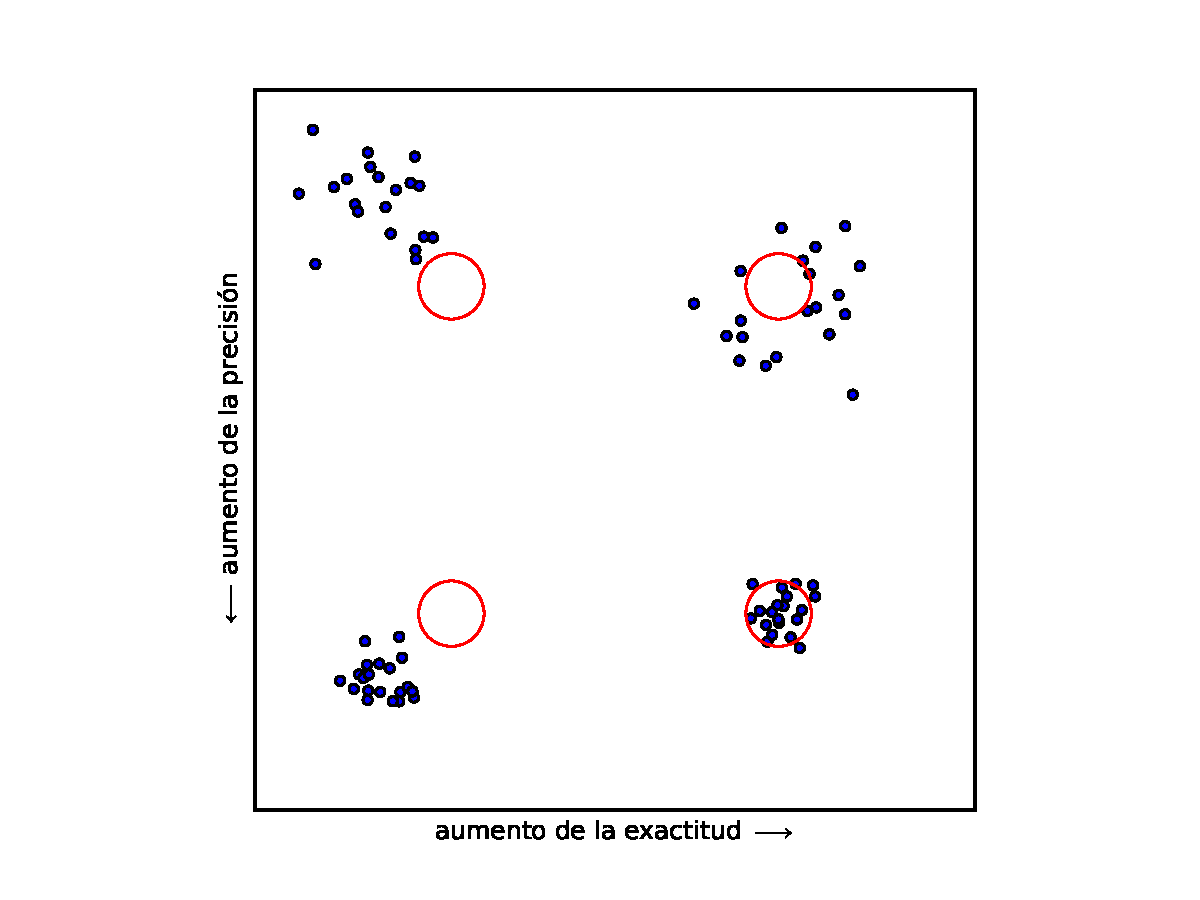
\includegraphics[width=12cm]{figs/fig-ex-vs-prec.pdf}
\caption{Exactitud versus precisi'on. C'odigo Python \href{https://github.com/gfrubi/Lab/blob/master/python/fig-ex-vs-prec.py}{aqu\'i}.}
\end{center}
\end{figure}

Asociado a los conceptos de precisi'on y exactitud est'a la idea de clasificar las fuentes de error en (al menos) tres tipos:
\begin{itemize}
\item \textbf{Error aleatorio}: La propiedad definitoria de los errores aleatorios es que 'estos producen resultados distintos al repetir una misma medici'on, incluso cuando se intentan dejar inalteradas todas las variables que determinan el resultado de 'este. Al repetir una medida varias veces, se obtienen diferentes resultados con una cierta dispersi'on. Esta dispersi'on determina entonces la precisi'on de los datos obtenidos. Como veremos, una medida de la dispersi'on de los datos, y por consiguiente de la precisi'on de la medida, es la \textbf{desviaci'on est'andar}. Las causas que producen el error aleatorio en un experimento son a menudo clasificadas como ``ruidos t'ecnicos"\, o ``ruidos fundamentales". Cada aparato tiene asociado un cierto l'imite de ruido fundamental determinado por la f'isica asociada a su funcionamiento. Sin embargo, usualmente el ruido t'ecnico es el dominante, y puede deberse a m'ultiples causas (mec'anicas, ambientales, variaciones en la forma en que se preparaci'on del sistema para repetir la medici'on... y un largo etc'etera!). Un(a) buen(a) f'isic@ experimental tiene experiencia y habilidad en identificar las posibles fuentes de ruido t'ecnico e idear formas de minimizarlo.

\item \textbf{Error sistem'atico}: Este tipo de error causa que los valores medidos se desplacen en alguna determinada direcci'on respecto al valor verdadero o aceptado. Por esto,  el error sistem'atico est'a relacionado con la exactitud del resultado: a mayor exactitud menor es el error sistem'atico. Las fuentes de este tipo de error pueden ser una defectuosa calibraci'on del instrumento de medici'on, o el uso de un m'etodo de medici'on que siempre sobre- o sub-estime la cantidad a determinar.

\item \textbf{Equivocaci'on}: Este tipo de error, en el que los m'etodos usados para estimar el error de una medida no son aplicables, se produce t'ipicamente porque alguna persona se equivoca en alguna de sus tareas. Por ejemplo, escribe mal el valor marcado en el instrumento al traspasarlo a su bit'acora (en papel, o en una planilla, o en un archivo con los datos, por ejemplo). Tambi'en puede ocurrir este tipo de error cuando la persona no ha chequeado correctamente la puesta en marcha de su instrumento, o que 'este est'e midiendo en una escala distinta, etc. etc. Si bien las equivocaciones pueden ser dif'iciles de distinguir de los errores sistem'aticos y aleatorios en la pr'actica, estos en principio no tienen relaci'on directa con el sistema f'isico, los instrumentos o el m'etodo usado, y en principio pueden ser eliminados repitiendo cuidadosamente el experimento.
\end{itemize}

En los gr'aficos de la figura \ref{fig-barras} se ilustra gr'aficamente las distintas posibilidades de error aleatorio y sistem'atico, por medio de \textbf{histogramas} (gr'aficos de barra de n'umero de ocurrencias de las medidas repetidas). En particular, suponemos que el valor verdadero de una variable es 10, y que medimos el valor de esta variable en repetidas oportunidades, para el caso simple en que nuestro instrumento nos suministre s'olo valores enteros.
\begin{figure}[h!]
\begin{center}
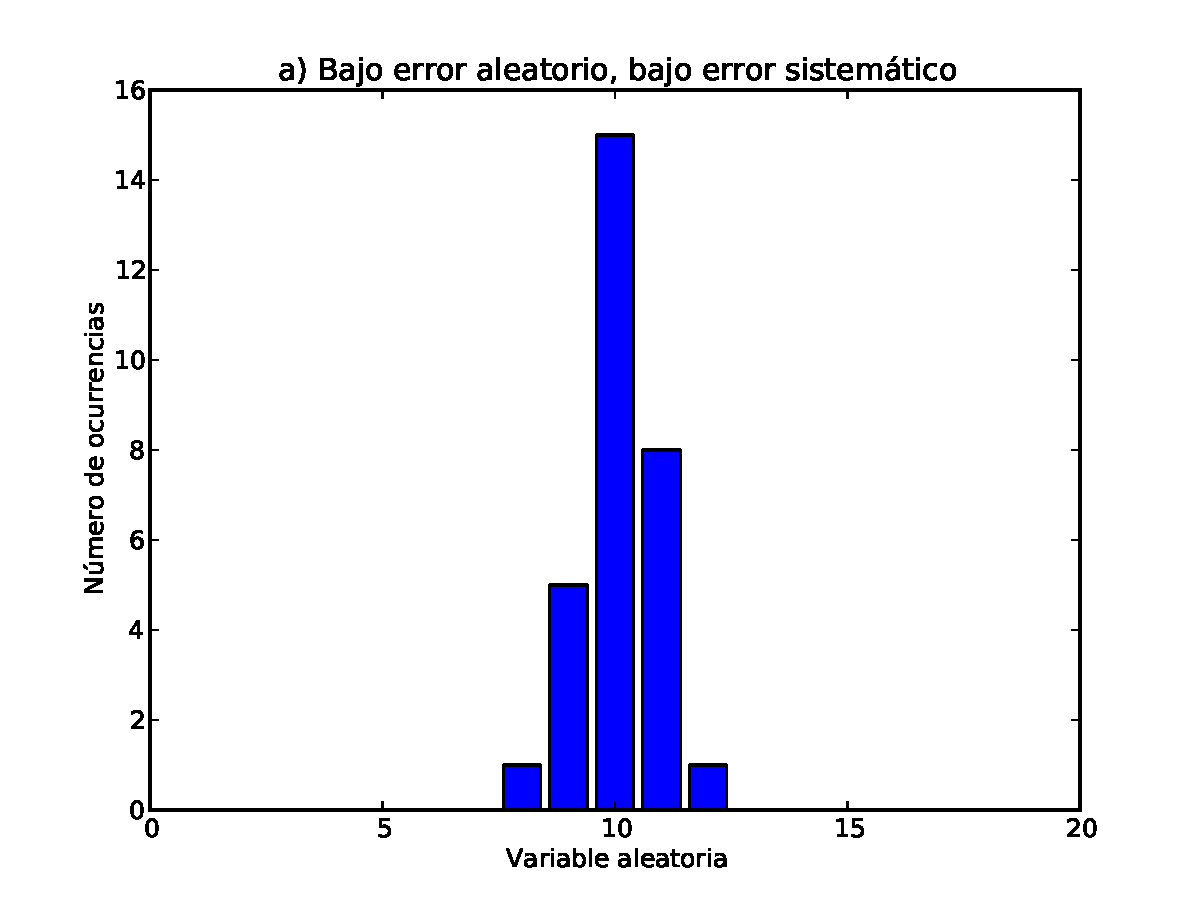
\includegraphics[width=7cm]{figs/fig-ba-bs.pdf}  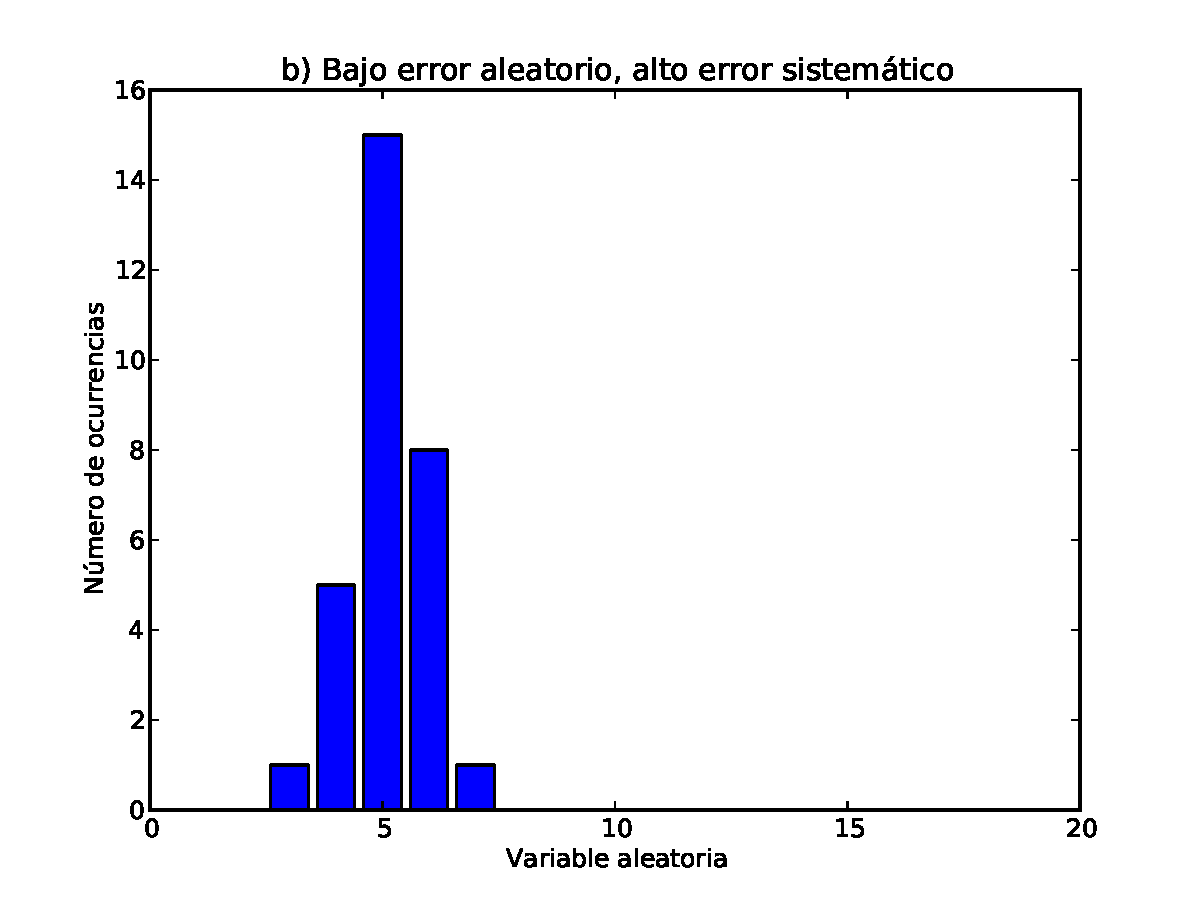
\includegraphics[width=7cm]{figs/fig-ba-as.pdf}
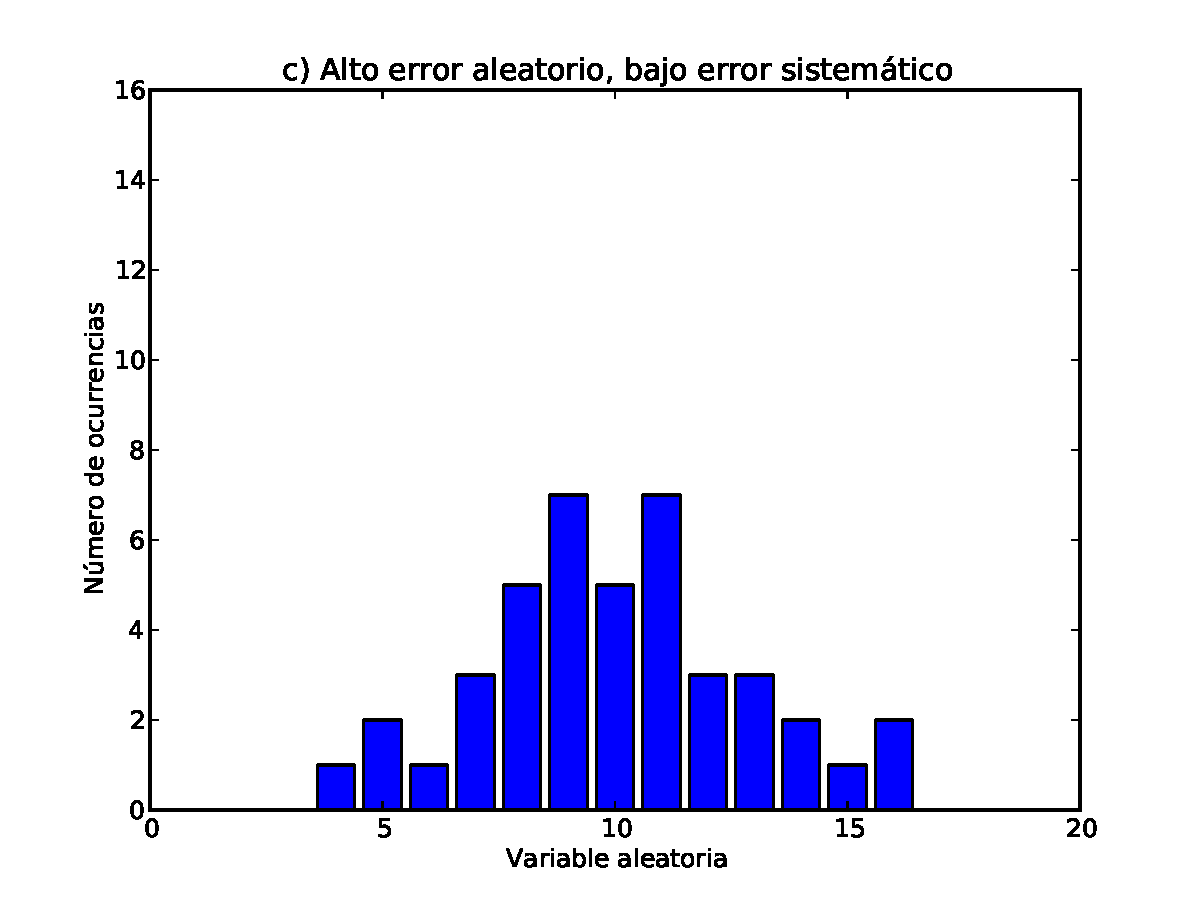
\includegraphics[width=7cm]{figs/fig-aa-bs.pdf}  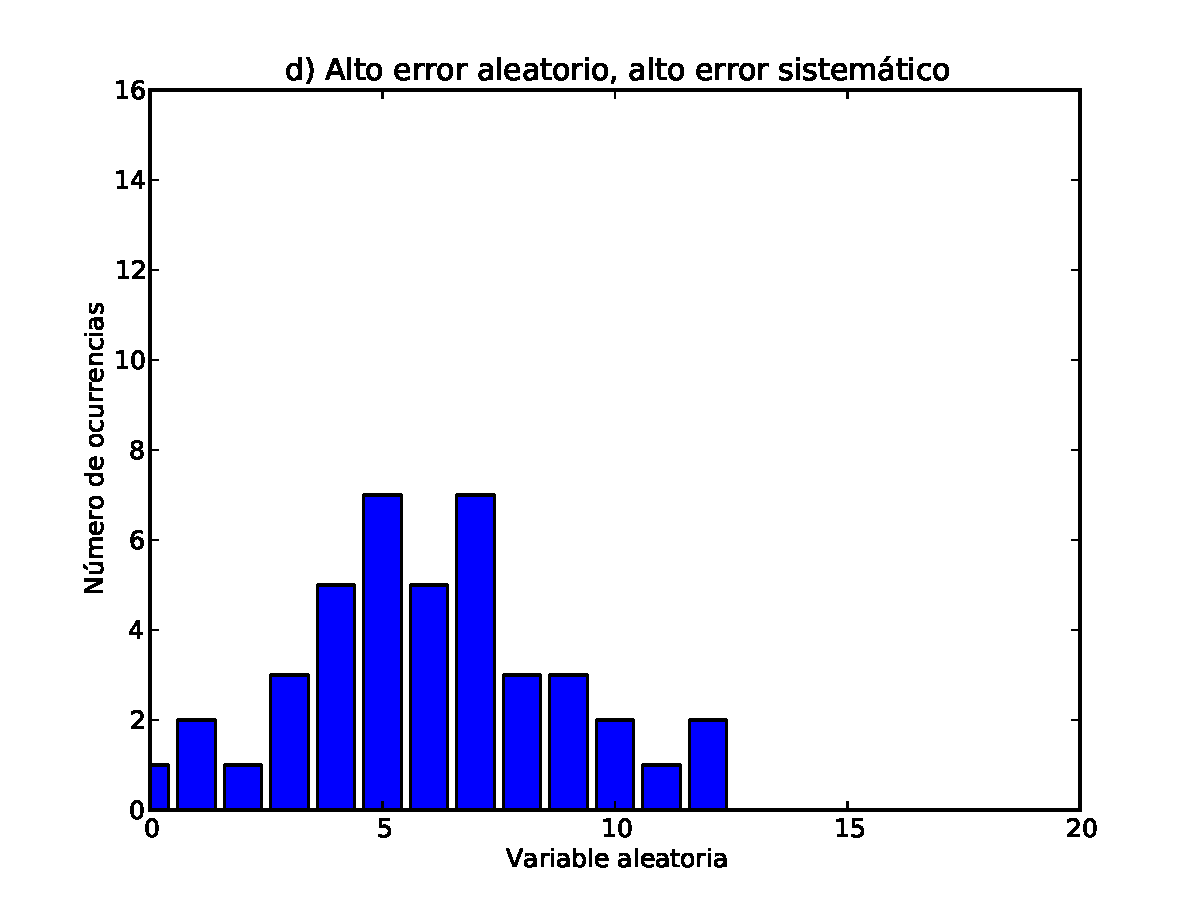
\includegraphics[width=7cm]{figs/fig-aa-as.pdf}
\caption{Distintas posibilidades para el tama\~no del error aleatorio y sistem'atico.  C'odigo Python \href{https://github.com/gfrubi/Lab/blob/master/python/fig-ba-bs.py}{aqu\'i}.}
\end{center}
\label{fig-barras}
\end{figure}


\section{Promedio y desviaci'on est'andar}

Cuando se realiza un experimento, generalmente se obtiene un conjunto de valores discretos $\lbrace x_i\rbrace$, $i=1,\dots,N$.  En el an'alisis de estos datos, a menudo son de gran utilidad los conceptos de \textbf{media}, \textbf{desviaci'on est'andar}, \textbf{varianza}, \textbf{error est'andar}, \textbf{suma residual de los cuadrados}  y la distribuci'on de los datos respecto del valor medio. 

La medida estad'istica m'as com'un es la \textbf{media}, definida como
\begin{equation}
\bar{x}:=\frac{1}{N}\sum_{i=1}^N x_i,
\end{equation}
donde $\lbrace x_i\rbrace$, $i=1,\dots,N$ representan los datos individuales y $N$ el n'umero total de 'estos.
Equivalentemente, podemos escribir
\begin{equation}
\bar{x}:=\frac{1}{N}\sum_{a=1}^{d} n_a x_a, \qquad N=\sum_{a=1}^{d} n_a,
\end{equation}
donde $n_a$ es el \textbf{n'umero de veces que se repite el valor} $x_a$ en la muestra y $d$ es el \textbf{n'umero de valores distintos} $\lbrace x_a\rbrace$, $a=1,\dots,d$.
%
%\begin{equation}
%\bar{y}:=\sum_{i=1}^N f_Y y_i,
%\end{equation}
%
%donde $ f_Y:= \frac{n_i}{N}$.
%
%\

La medida m'as com'un de la variabilidad de un conjunto de datos, es la \textbf{desviaci'on est'andar} respecto a la media:
\begin{equation}
s:=\sqrt{\frac{1}{N-1}\sum_{i=1}^N(x_i-\bar{x})^2}.
\end{equation}
Otro s'imbolo usando para la misma cantidad es $\sigma_{N-1}$, ver por ejemplo \cite{HH2010}. En Python, puede calcular la desviaci'on est'andar definida arriba usando la funci'on \texttt{std} de Numpy, con la opci'on \texttt{ddof=1}. Por ejemplo, \texttt{np.std(x, ddof=1)}.

Otro estimador de la variabilidad, el \textbf{error estándar}, es definido por:
\begin{equation}
\alpha:=\frac{s}{\sqrt{N}}.
\end{equation}
Si la dispersi'on de los datos respecto a la media aumenta, $s$, y $\alpha$ crecen. Por otro lado, si las medidas individuales est'an muy cerca del valor medio, estas cantidades ser'an menores. La dispersi'on tambi'en puede representarse por una magnitud llamada \textbf{varianza}, que por definici'on es el cuadrado de la desviaci'on est'andar,
\begin{equation}
s^2=\frac{1}{N-1}\sum_{i=1}^N(x_i-\bar{x})^2.
\end{equation}

 El valor del denominador, $N-1$ en lugar de $N$ se elige debido a que s'olo existen $N-1$ variaciones \textit{independientes} $(x_i-\bar{x})$, ya que $\sum_{i=1}^N (x_i-\bar{x})\equiv 0$. Formalmente decimos que se pierde un grado de libertad. Otra justificaci'on es que la dispersi'on no est'a definida en caso de tener s'olo un dato (en ese caso se obtiene $0/0$).

En t'erminos de los valores distintos $\lbrace x_a\rbrace$, y de su correspondiente n'umero de repeticiones $\lbrace n_a\rbrace$, podemos escribir la varianza como
\begin{equation}
s^2=\frac{1}{N-1}\sum_{a=1}^{d}n_a(x_a-\bar{x})^2.
\end{equation}

%Otra medida estad'istica que es 'util para cuantificar la dispersi'on es el \textbf{coeficiente de variaci'on}, definido por:
%\begin{equation}
%c.v.:=\frac{s}{\bar{x}}\times 100\%.
%\end{equation}
%
%\textbf{Suma residual}, es la suma de las diferencias al cuadrado entre el modelo predictor y los datos medidos.
%\begin{equation}
%\xhi^2:=\sum_{i=1}^N(y_i-f(x_i))^2.
%\end{equation}
%donde la funci'on $f(x_i)$ es el modelo usado para predecir los valores de $y_i$.


\section{Cifras significativas}

Al expresar una cierta magnitud f'isica, decimos que su valor tiene un cierto n'umero de \textbf{cifras significativas}, es decir, un cierto n'umero de d'igitos que, tomando en cuenta la incertidumbre en la determinaci'on de su valor, entregan informaci'on relevante del valor de la magnitud en cuesti'on. Las cifras significativas pueden t'ipicamente dividirse en cifras de las que se est'a completamente seguro, y en cifras que si bien no se tiene certeza absoluta de su valor, suministran informaci'on relavante para estimar el valor de la magnitud. Por ejemplo, la constante gravitacional en \eqref{G} fue expresada usando 6 cifras significativas ($6, 6, 7, 3, 8$ y $4$). Dada la incertidumbre en el valor de esta constante universal, s'olo las tres primeras cifras son seguras, mientras que las 'ultimas tres pueden cambiar. Sin embargo, en ese caso se ha considerado que las tres cifras no seguras tambi'en tienen informaci'on relavante de ser reportada. En general, no existe una regla absoluta y universamente aceptada sobre c'omo definir el n'umero de cifras significativas que es necesario o 'util de considerar al reportar un cierto resultado experimental. Por contraste, las siguientes reglas son univesalmente aceptadas para definir \textit{cifras que no son significativas}:
\begin{itemize}
\item Todos los ceros a la izquierda de una cantidad.
\item Ceros a la derecha de una cantidad, en el caso en que 'estos indican solamente la escala del n'umero (y/o las unidades de medida usadas).
\item Cifras espurias que aparezcan producto de c'alculos que van m'as all'a de la precisi'on que los datos originales determinan y que por este motivo no suministren ninguna informaci'on f'isicamente relevante de la magnitud.
\end{itemize}

En el caso en que un cero a la derecha de una cantidad se considere como significativo (es decir, que suministra informaci'on relavante, ya sea porque es una cifra segura o porque si bien no es segura es la cifra que se considera m'as probable) se acostumbra a escribir esa cifra expl'icitamente. Por ejemplo, si decimos que una distancia es $x_1=1,70{\rm\, km}$, estamos expresando que las cifras $1$ y $7$ y $0$ son significativas, mientras que si escribimos $x_2=1,7{\rm\, km}$ estamos indicando que s'olo 2 cifras son consideradas significativas. Si quieremos expresar las mismas cantidades, pero en unidades de metros y no kil'ometros, se acostumbra entonces escribir $x_1=1,70\times 10^3{\rm\, m}$ (3 cifras significativas) y $x_2=1,7\times 10^3{\rm\, m}$ (2 cifras significativas), respectivamente.

Ejemplos:

\begin{equation}
\begin{array}{ll}
2 & (1 \text{ cifra significativa)}\\
32 & (2 \text{ cifras significativas)}\\
12,470 & (5 \text{ cifras significativas)}\\
12,0010 &(6 \text{ cifras significativas)}\\
0,0023 & (2 \text{ cifras significativas)}\\
000156,210 & (6 \text{ cifras significativas)}\\
2,3\times 10^5 &(2 \text{ cifras significativas)}
\end{array}
\end{equation}


\subsubsection{Ejercicio}

Un(a) estudiante mide el largo de una mesa y como resultado nos entrega
la siguiente cantidad $(2,1\pm 0,5)$ m. Este(a) estudiante, por
conveniencia, decide expresar su resultado en mil'imetros. ?`C'omo tendr'ia
que expresar su resultado?, ?`$(2100\pm 50)$ mm?. \textbf{Resp.:} No, puesto que esto dar'ia a entender que la cantidad fue expresada con 4 cifras significativas, cuando en realidad s'olo tiene 2. La convenci'on para expresar el resultado es: $(2,1\pm 0,5)\times 10^3\,\rm mm$.

\section{Aproximaci'on y Redondeo}

Si queremos expresar el n'umero $\pi=3,14159265358979\cdots$ con $n$
cifras significativas, debemos desechar todas las cifras que se
encuentren a la derecha del en'esimo lugar. Adem'as, se adoptan las siguientes reglas para \emph{redondear} la $n$-'esima cifra:
\begin{enumerate}
\item Si la cifra que se encuentra en el lugar $(n + 1)$ es mayor que 5, se
  le agrega una unidad a la cifra que se encuentra en el lugar en'esimo.
\item Si la cifra que se encuentra en el lugar $(n + 1)$ es menor que 5,
  dejamos la cifra en'esima inalterable.
\item Si la cifra que se encuentra en el lugar $(n + 1)$ es igual a 5,
  adoptaremos la siguiente \textit{convenci'on}:
	\begin{itemize}
	\item Si la en'esima cifra es impar, se le agrega una unidad.
	\item Si la en'esima cifra es par la dejamos inalterable.
	\end{itemize}
Esta convenci'on intenta evitar la introducci'on del error sistem'atico que se agregar'ia si, por ejemplo, redondearamos siempre ``hacia arriba"\, la $n$-'esima cifra. En Python, estas reglas están implementadas en la función \texttt{round} de Numpy, ver \href{https://docs.scipy.org/doc/numpy/reference/generated/numpy.round_.html}{la documentaci\'on}.
\end{enumerate}

Note que estas convenciones de redondeo se aplican al valor principal de una magnitud f'isica y no al error asociado, puesto que este 'ultimo siempre se redondea a la cifra superior.

\section{Orden de magnitud}
Es la potencia de diez m'as cercana. 
Ejemplos:
\begin{itemize}
\item $6.7$ es de orden $10^1$ (est'a m'as cerca de 10 que de 1).
\item $5.3$ es de orden $10^0$ (est'a m'as cerca de 1 que de 10).
\item $128.9$ es de orden $10^2$ (est'a m'as cerca de 100 que de 1000).
\end{itemize}






\section{Precisi'on, sensibilidad, y cifras significativas}

En F'isica (y otras ciencias), estamos especialmente interesad@s en distinguir las cifras que son relevantes a la hora de expresar el resultado de una cantidad f'isica, de las que no lo son, \textit{a partir de la precisi'on con la que medimos o calculamos la cantidad} en cuesti'on. Por ejemplo, si medimos una 'unica vez el ancho de una hoja con una regla (o similar) que tiene una escala con una graduaci'on m'inima de un mil'imetro (decimos que la \textbf{sensibilidad del instrumento} es un 1\,mm), y vemos que el valor buscado est'a en la zona interior entre las marcas de la regla correspondientes a $21.5\,\rm cm$ y $21.6\,\rm cm$, podr'iamos expresar el resultado con 4 cifras significativas: $(21.55\pm 0.05)\,\rm cm$, o bien $(215.5\pm 0.5)\,\rm mm$. En este caso, la 'ultima cifra considerada como significativa es \textit{estimada}, es decir, aproximada por el criterio de la persona que realiza la medida. En este ejemplo, siendo conservadores (o pesimistas) aseguraremos que (con 100\% de confianza), el ancho de la hoja est'a comprendido en el intervalo entre $21.5\,\rm cm$ y $21.6\,\rm cm$ de modo que (en el peor de los casos) tendremos 2 cifras seguras ($2$ y $1$) y dos cifras que podr'ian variar, pero que nos entregan informaci'on f'isica relevante a la medici'on. Por el contrario, en este tipo de medici'on no tiene ning'un sentido f'isico reportar que el ancho de la hoja, medido con la misma regla, es $21.55275165359\,\rm cm$ puesto que las cifras $275165359$ no son para nada confiables (la cifra anterior, $5$, ya corresponde a una estimaci'on que realiz'o la persona que realiz'o la medida). En general, toda cifra que est'a m'as a la derecha de la posici'on que la precisi'on de la medida determina es considerada como no significativa (a menos que existen muy buenos argumentos para considerar lo contrario!).

Para estimar la precisi'on que determina (entre otras cosas) el n'umero de cifras significativas con las que se reporta un resultado o, equivalentemente el error o incertidumbre de la medida es 'util considerar varios casos:

\subsection{Caso de una 'unica medici'on}
En este caso se hace, a su vez, la distinci'on entre:
\begin{itemize}
\item \textbf{Medici'on realizada con un instrumento anal'ogico}: Aqu'i decimos que la sensibilidad del instrumento es el valor de la m'inima subdivisi'on en la escala que 'este posee. Para la regla considerada en el ejemplo anterior, decimos que su sensibilidad es 1\,mm. Es razonable considerar la incertidumbre o error de una medida realizada con un instrumento anal'ogico como la mitad del valor de su sensibilidad: 0.5\,mm en el caso de la regla. Esta es la ``elecci'on conservadora''\, para el error de la medida\footnote{En algunas ocasiones, sin embargo, esta elecci'on puede ser claramente demasiado pesimista. Considere por ejemplo que se mide el mismo ancho de la hoja, pero con una regla que tenga una sensibilidad de 1\,cm (la menor graduaci'on marcada en ella). En este caso la medida quedar'a entre 21\,cm y 22\,cm, y el error ``conservador''\, asociado ser'ia de $\pm 0.5\,\rm cm$, pudiendo expresar el resultado como $(21.5\pm 0.5)\rm cm$ que, al ojo humano sano, puede parecer muy pesimista. Un(a) f'isic(a) experimental con experiencia y habilidad podr'ia ser capaz de realizar una mejor estimaci'on de la 'ultima cifra y acotar el error asociado asegurando, por ejemplo, que el ancho est'a entre $21.1\,\rm cm$ y $21.7\,\rm cm$ y por lo tanto informe que $(21.4\pm 0.3)\rm cm$. Dado que no existe una receta general y 100\% aceptada de c'omo proceder en estos casos (que aseguren que las personas que reciben el resultado tengan confianza en 'el), adoptaremos aqu'i la postura ``pesimista'', es decir, consideraremos que el error de una medici'on es igual a la mitad de la sensibilidad del instrumento.}

\item \textbf{Medici'on realizada con un instrumento digital}: Suponga que mide el mismo ancho de la hoja, pero ahora usando un instrumento digital\footnote{?`C'omo podr'ia hacer esto?, ?`Con qu'e instrumento?}), que suministra valores discretos en una pantalla, por ejemplo ``21.57''\,cm. ?`Qu'e error asociamos a la medida?. Nuevamente, la respuesta no es 'unica, puesto que depende de c'omo exactamente funciona el dispositivo, y de c'omo realiza el redondeo y/o truncamiento de cifras que finalmente son mostradas en la pantalla. Algunos instrumentos digitales traen consigo especificaciones t'ecnicas del fabricante que establecen que el error debe considerarse como ``la mitad del 'ultimo d'igito''\,. En nuestro ejemplo reportar'iamos entonces que el ancho es $(21.570\pm 0.005)\rm cm$ (el 'ultimo 0 ser'ia una cifra significativa en este caso) o, equivalentemente, que el valor est'a en el intervalo entre $21.565\,\rm cm$ y $21.575\,\rm cm$. Como podemos ver, este caso requiere que el instrumento (internamente) \textbf{redondee} (aproxime) el valor de la medida, y que no simplemente \textbf{trunque} (corte) el valor. En el caso que se desconozcan los detalles t'ecnicos del instrumento y/o si 'este aproxima o trunca las cifras es preferible, nuevamente, adoptar la postura ``conservadora''\, y considerar como error de la medida a la unidad correspondiente al 'ultimo d'igito que el instrumento indica. En nuestro ejemplo, $\pm 0.01\rm cm$, y reportar que $(21.57\pm 0.01)\rm cm$.
\end{itemize}

\subsection{Caso de mediciones repetidas}

En este caso, es necesario a recurrir a herramientas estad'isticas para caracterizar algunos aspectos de la precisi'on de los resultados, puesto que es esencial tomar en cuenta que se realizan varias (idealmente, muchas) medidas, y que 'estas en general no arrojar'an los mismos valores, por lo que los datos estudiados tendr'an cierta dispersi'on. Existen distintas cantidades que son 'utiles para caracterizar el valor caracter'istico y la dispersi'on en los datos, pero que necesariamente reducen la riqueza y complejidad 'estos. Teniendo esto en cuenta, es posible usar (por ejemplo) el promedio ($\bar{x}$) y la desviaci'on est'andar ($\sigma$) (es decir, s'olo dos valores!) para expresar el valor caracter'istico y el ``error'' de una magnitud f'isica que queremos determinar a partir de muchas medidas individuales. Hay, sin embargo, un precio que pagar: es necesario incluir adem'as un valor para la \textbf{probabilidad de que el valor buscado est'e dentro de cierto intervalo} (por ejemplo, $\bar{x}\pm \sigma$).

\section{Propagaci'on de incertezas}

Inevitablemente, siempre que calculemos una magnitud f'isica a partir de otras sujetas a incerteza/error, 'esta incerteza se propagar'a a la cantidad calculada. Existen varias formas de calcular la incerteza de la magnitud calculada a partir de la expresi'on anal'itica que la define y de  incertezas de las magnitudes originales. Si la relaci'on es simple es posible encontrar expresiones anal'iticas exactas para el error propagado. En otros casos tambi'en es posible encontrar expresiones anal'iticas aproximadas cuando el error de las magnitudes originales es suficientemente peque\~no. Actualmente es tambi'en muy com'un evaluar num'ericamente el error propagado, puesto que este m'etodo puede ser usado cuando la relaci'on entre las variables en muy complicada y adem'as cuando el error no necesariamente es peque\~no.

Un caso simple donde es posible encontrar una expresi'on anal'itica exacta para el error propagado es en el caso de la suma y resta de dos magnitudes:
\begin{itemize}
\item \textbf{Suma:} Si $y=x_1+x_2$, $x_1 = \bar{x}_1\pm\Delta x_1$ y $x_2 = \bar{x}_2\pm\Delta x_2$, entonces
\begin{equation}
\bar{y}= \bar{x}_1+\bar{x}_2, \qquad  \Delta y= \Delta x_1+\Delta x_2.
\end{equation}
\item \textbf{Resta:} Si $y=x_1-x_2$, entonces
\begin{equation}
\bar{y}= \bar{x}_1-\bar{x}_2, \qquad  \Delta y = \Delta x_1+\Delta x_2.
\end{equation}
\end{itemize}

En el caso de la multiplicaci'on y divisi'on la situaci'on es menos simple:
\begin{itemize}
\item \textbf{Multiplicaci'on:} Si $y=x_1 x_2$, (y suponiendo $x_1$ y $x_2$ positivos)
\begin{equation}
y_{\rm min} = (\bar{x}_1-\Delta x_1)(\bar{x}_2-\Delta x_2), \qquad 
y_{\rm max} = (\bar{x}_1+\Delta x_1)(\bar{x}_2+\Delta x_2).
\end{equation}
Vemos aqu'i que el punto medio no coincide con el valor que se obtendr'ia sin considerar el error, ya que
\begin{equation}
\frac{1}{2}\left(y_{\rm min}+y_{\rm max}\right) = \bar{x}_1\bar{x}_2+\Delta x_1\Delta x_2,
\end{equation}
en otras palabras, el intervalo $[y_{\rm min},y_{\rm max}]$ no es sim'etrico respecto a $\bar{x}_1\bar{x}_2$.

Esta asimetr'ia puede ignorarse si los errores relativos de $x_1$ y $x_2$ son suficientemente peque\~nos, de modo que $u_r^{x_1}\ll 1$ y $u_r^{x_2}\ll 1$. En este caso,
\begin{equation}
\frac{1}{2}\left(y_{\rm min}+y_{\rm max}\right) \approx \bar{x}_1\bar{x}_2,
\end{equation}
y podemos expresar el valor de $y$ como $\bar{y}\pm\Delta y$, con
\begin{equation}
\bar{y} \approx \bar{x}_1\bar{x}_2, \qquad  \Delta y= x_2\Delta x_1 + x_1\Delta x_2 , 
\end{equation}
o, equivalentemente,
\begin{equation}
u_r^{y} \approx u_r^{x_1} + u_r^{x_2}.
\end{equation}

\item \textbf{Divisi'on:} Si $y=x_1/x_2$, y suponiendo $x_1$ y $x_2$ positivos, tendremos una situaci'on similar. Los valores extremos estar'an dados por
\begin{equation}
y_{\rm min} = \frac{\bar{x}_1-\Delta x_1}{\bar{x}_2+\Delta x_2}, \qquad 
y_{\rm max} = \frac{\bar{x}_1+\Delta x_1}{\bar{x}_2-\Delta x_2},
\end{equation}
por lo que el valor medio y el ancho del intervalo son dados por
\begin{equation}
\frac{1}{2}\left(y_{\rm min}+y_{\rm max}\right) = \frac{\bar{x}_1\bar{x}_2+\Delta x_1\Delta x_2}{\bar{x}_2^2-(\Delta x_2)^2}, 
\qquad \frac{1}{2}\left(y_{\rm max}-y_{\rm min}\right) = \frac{\bar{x}_2\Delta x_1 + \bar{x}_1\Delta x_2}{\bar{x}_1^2-(\Delta x_1)^2}.
\end{equation}
El punto medio s'olo coincide aproximadamente con el valor $\bar{x}_1/\bar{x}_2$ si el error (relativo) es muy peque\~no. Suponiendo que esto es cierto, podremos escribir $y = \bar{y}\pm\Delta y$, con
\begin{equation}
\bar{y}\approx \frac{\bar{x}_1}{\bar{x}_2}, \qquad  \Delta y \approx \frac{1}{x_2}\Delta x_1 + \frac{x_1}{x_2^2}\Delta x_2
\end{equation}
o, equivalentemente,
\begin{equation}
u_r^{y} \approx  u_r^{x_1} + u_r^{x_2}.
\end{equation}

\item \textbf{Potencias:} Es simple generalizar los resultados anteriores al caso en que $y=x_1^{\alpha_1} x_2^{\alpha_2}$, el intervalo de valores posibles de $y$ tampoco ser'a sim'etrico respecto al valor calculado sin tomar en cuenta los errores de cada variable: $\bar{y}=\bar{x}_1^{\alpha_1}\bar{x}_2^{\alpha_2}$. Sin embargo, en el caso en que los errores relativos satisfagan $u_r^{x_1}\ll 1$ y $u_r^{x_2}\ll 1$ podremos escribir
\begin{equation}
\bar{y}\approx \bar{x}_1^{\alpha_1}\bar{x}_2^{\alpha_2}, \qquad  u_r^{y} \approx  |\alpha_1|u_r^{x_1} + |\alpha_2|u_r^{x_2}.
\end{equation}
\end{itemize}


\paragraph{Ejemplo:}
 Suponga que determinamos el volumen de un gas a partir de la ecuaci'on para un gas ideal,
\begin{equation}
V(p,T,n,R)=\frac{nRT}{p},
\end{equation}
donde cada magnitud f'isica es medida con su respectivo error asociado:
\begin{equation}
p=(100\pm 3)\times 10^3\text{ Pa}, \quad T=(300.0\pm 0.2)\text{ K}, 
\quad n=(0.10\pm 0.01)\text{ mol},
\end{equation}
mientras que de una tabla de datos se obtiene
\begin{equation}
R=(8.31\pm 0.01)\text{ J/mol K}.
\end{equation}
El valor principal del volumen:
\begin{equation}
\bar{V}= V(\bar{p},\bar{T},\bar{n},\bar{R}) \approx 0.002493\text{ m}^3.
\end{equation}
Ahora evaluaremos el error relativo asociado con el volumen, usando
\begin{align}
u_r^V &\approx u_r^n+ u_r^R + u_r^T + u_r^p \\
&\approx \frac{0.01}{0.1} + \frac{0.01}{8.31} + \frac{0.2}{300} + \frac{3}{100} \\
&\approx 0.1 + 0.0012 + 0.00067 + 0.03 \\
&\approx 0.132.
\end{align}
Con esto, el error absoluto $\Delta V$ queda determinado por
\begin{equation}
\Delta V = \bar{V}u_r^V \approx (0.002493\text{ m}^3)(0.13) \approx 3.3\times 10^{-4}\text{ m}^3.
\end{equation}
Tomando en cuenta el error calculado, expresamos el resultado final truncando el valor de $\bar{V}$ de acuerdo a las reglas antes descritas:
\begin{equation}
 V \approx (0.002493\pm 0.00033)\text{ m}^3 \approx (2.49\pm 0.33)\times 10^{-3}\text{ m}^3.
 \end{equation} 

\paragraph{Ejemplo:}
Supongamos que queremos medir el periodo de un p'endulo y, medimos el tiempo que tarda en hacer 10 oscilaciones, con un cron'ometro (digital) de sensibilidad $0.1\,\rm s$. Si el tiempo total es de $t=(4.6\pm 0.1)\,\rm s$, tendremos que el periodo medio es 
\begin{equation}
\bar{P} = \frac{\bar{t}}{10}=\frac{4.6\,\rm s}{10}=0.46{\,\rm s}.
\end{equation}
Y el error puede ser estimado usando
\begin{equation}
\Delta P = \frac{0.1\,\rm s}{10}=0.01{\,\rm s},
\end{equation}
de modo que
\begin{equation}
P=(0.46\pm 0.01){\,\rm s}.
\end{equation}

Note que por el solo hecho de haber medido el tiempo de 10 oscilaciones consecutivas y haber calculado a partir de 'este el tiempo de una 'unica oscilaci'on parece que hemos aumentado la precisi'on de la medida, tal como si us'aramos un instrumento 10 veces m'as sensible. Si bien este m'etodo es apropiado y usado en muchas ocasiones, existe un ``precio que pagar'' por este aumento efectivo de la precisi'on: \textit{hemos supuesto que el periodo de oscilaci'on del p'endulo durante las 10 oscilaciones permanece inalterado}. Esta es una hip'otesis f'isica adicional introducida, que puede o no ser cierta. En otras palabras, si el periodo de oscilaci'on del p'endulo no permanece constante durante las 10 oscilaciones, la cantidad calculada es simplemente el valor promedio de los periodos y no necesariamente el valor que se busca determinar.

\paragraph{Ejemplo:}
La ley de gravitaci'on universal de Newton, determina la fuerza $\vec{F}$ entre dos masas (muy peque\~nas) $m_1$ y $m_2$ separadas por una distancia $d$, de modo que $
F=G{m_1m_2}/{d^2}$. En un experimento se quiere determinar la constante gravitacional con un error relativo $u_G\approx 10^{-3}$, usando 
\begin{equation}
G=\frac{Fd^2}{m_1m_2}.
\end{equation}
Para esto, se ubican dos masas iguales $m_1=m_2=(100{\,\rm kg}\pm 1{\,\rm g})$ a una distancia $d\approx 0.5{\, \rm m}$, y se mide la fuerza entre las masas, con un error relativo $u_F=2\times 10^{-4}$. Determine el error absoluto con el que deben medirse la distancia $d$ que el error relativo de $G$ sea el deseado.

\textbf{Soluci'on:} En este caso, los errores relativos conocidos son mucho menores que 1, ya que
\begin{equation}
u_r^F =2\times 10^{-4}, \qquad u_r^m = \frac{1\,\rm g}{100\,\rm kg}  = 10^{-5}, \qquad u_r^G\approx 10^{-3},
\end{equation}
de modo que podemos usar la expresion aproximada para el error relativo propagado:
\begin{equation}
u_r^G \approx u_r^F + 2u_r^d + 2u_r^m.
\end{equation}
Despejando $u_r^d$, obtenemos
\begin{align}
u_r^d &\approx \frac{1}{2}\left(u_r^G - 2u_r^F - 2u_r^m\right) \\
& \approx\frac{1}{2}\left(10^{-3} - 4\times 10^{-4} - 2\times 10^{-5}\right) \\
& \approx 4\times 10^{-4}.
\end{align}
El valor del error absoluto de las medidas de $d$ debe entonces ser aproximadamente de $\Delta r = r\cdot u_r^r \approx (0.5 m)(4\times 10^{-4})\approx 0.2\,\rm mm$.

\subsection{Funciones arbitrarias y error suficientemente peque\~no}

Si $y=y(x)$, y $x=\bar{x}\pm \Delta x$ entonces
\begin{equation}
\Delta y \approx \Delta x \left|\frac{dy}{dx}(\bar{x})\right|.
\end{equation}

Si $y=y(x_1,x_2,\dots,x_m)$, y $x_\alpha=\bar{x}_\alpha\pm \Delta x_\alpha$, $\alpha=1,\dots, m$ entonces
\begin{equation}
\Delta y \approx \sum_{\alpha=1}^m\Delta x_\alpha \left|\frac{\partial y}{\partial x_\alpha}(\bar{x}_1,\dots,\bar{x}_m)\right|.
\end{equation}

\subsection{Evaluaci'on num'erica}
